\chapter{Systembeskrivelse (MK PO)}

EasyWater8000 er et samlet vandingssystem, hovedsagligt målrettet imod vanding af en golfbane. Her følger en detaljeret beskrivelse af systemet.

\begin{figure}[H]
  \centering
    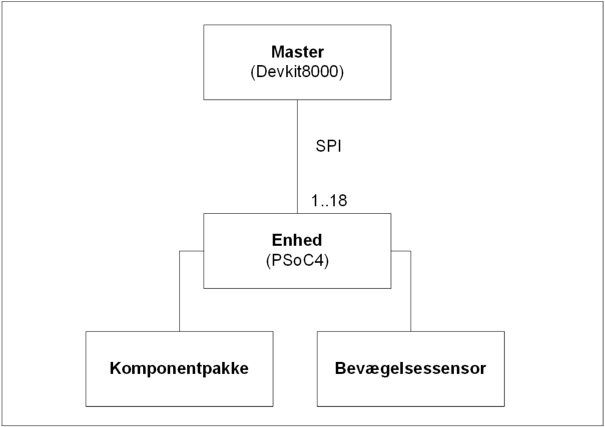
\includegraphics[width=0.9\textwidth]{billeder/systembeskrivelse}
    \caption{Oversigt over det samlede system}
    \label{fig:systembeskrivelse}
\end{figure}

Figur \ref{fig:systembeskrivelse} viser et simplificeret overblik over hvad EasyWater8000 består af. Der er en Master, som er hovedcomputeren i systemet med Linux(Angstrom) som styresystem. Masteren kommunikerer og styrer op til 18 Enheder der hver har en komponentpakke og en bevægelsessensor tilsluttet.

Komponentpakken er en samling af 3 komponenter, en temperatursensor og en fugtsensor til at hhv. måle temperaturen og fugtigheden i jorden omkring komponentpakken, samt en sprinkler til at vande græsset og jorden i samme område.

Bevægelsessensoren sidder ved hvert teested på golfbanen, og registrerer bevægelse i det område. Når der bliver registreret bevægelse vil sensoren give signal til at deaktivere vandingen på det givne golfhul, så golfspillerne ikke bliver utilsigtet våde.

Et golfhul kunne se ud som på Figur \ref{fig:hul_med_sprinkler}

\begin{figure}[H]
  \centering
    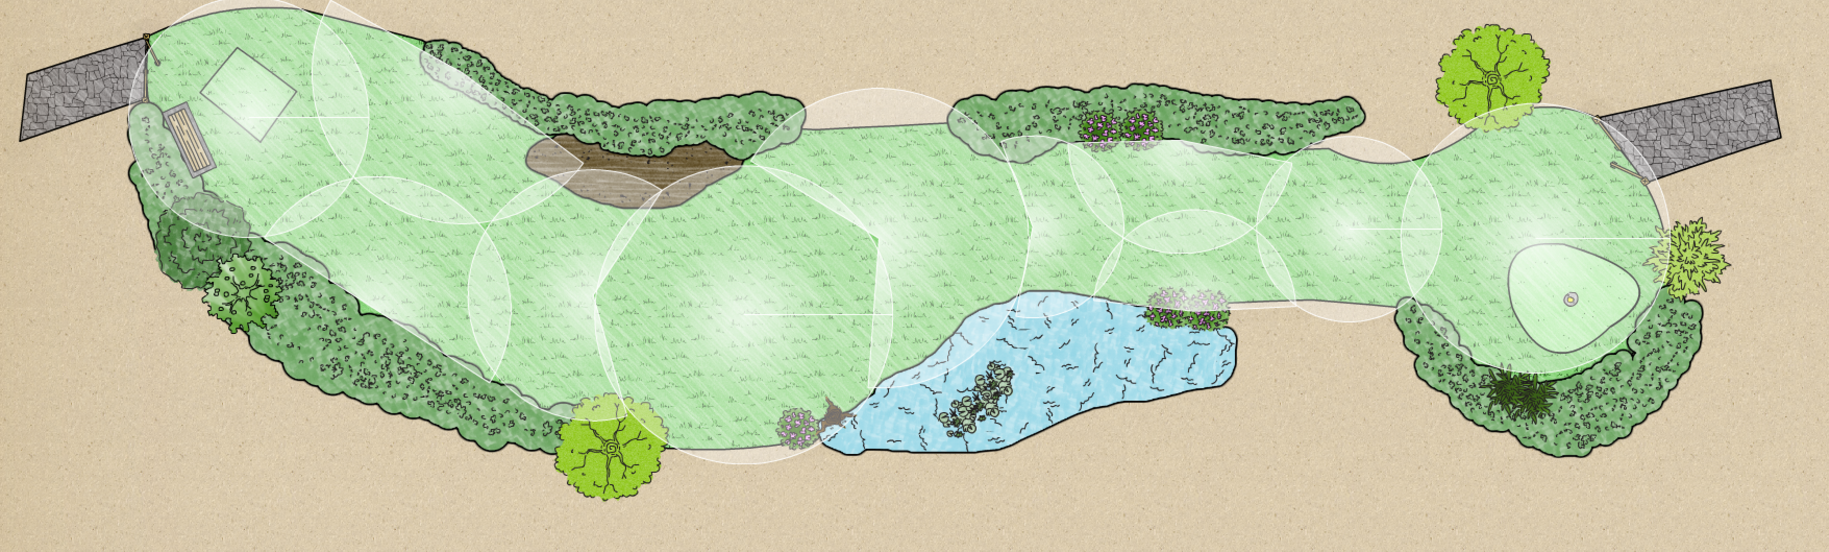
\includegraphics[width=\textwidth]{billeder/hul_med_sprinkler}
    \caption{Eksempel på golfbane med sprinklere}
    \label{fig:hul_med_sprinkler}
\end{figure}

Enhederne kører autonomt, dvs. de selv monitorerer fugt og temperatur og vander hvis grænserne overskrides. Enhederne får deres grænseværdier fra Masteren og logger sine målte data til Masteren, via SPI transmission.